\makeatletter
\def\input@path{{../}}
\makeatother
\documentclass[../main.tex]{subfiles}
\graphicspath{
  {"../images/03/"}
  {"./images/03/"}
}

\begin{document}
\chapter{Probability Distributions}
\section{Random Variables}
\begin{definition}
A \textbf{random variable} is a function $X : \Omega \rightarrow R$. It assigns a real number to each outcome. 
\end{definition}
(In other words, a random variable is like a vending machine- it dispenses numbers according to a possibly unknown function.)

A random variable $X$ might output some concrete number $x$, with some probability. If this probability is $\frac 12$, then we write this
\[
	\Pr[X = x] = \frac 12
\]
For the sake of continuing the ``vending machine'' analogy, we will temporarily say \[\Pr[X \hookrightarrow x] = \frac 12,\] where $\hookrightarrow$ is pronounced ``dispenses,'' i.e. $X$ dispenses $x$ with probability $\frac 12$. 

\subsection{Probability Mass Function}

These random variables have probabilities associated with them, just as
outcomes and events in the sample space. The probability function
associated with a discrete random variable is called a \textbf{probability
mass function}
\begin{definition}
    A \textbf{probability mass function} (pmf) is a function  $f:\RR \rightarrow [0,1]$ from the reals to the unit interval such that $f(x) = \Pr[X \dsp x]$, that is the probability that
    a random variable dispenses a given value. It must satisfy the following criteria
    \begin{enumerate}
        \item $\displaystyle \sum_{x_i} f(x_i) = 1$, where the sum is over
        every $x_i$ in the range of $X$.
        \item $f(x_i) = 0$ for every $x_i$ not in the range of $X$.
    \end{enumerate}
\end{definition}
We will elucidate these ideas with a number of examples
\begin{example}
    Let a 6-sided die be constructed such that the probability of rolling
    a 4 is twice that of rolling any other value. Describe this in terms
    of a random variable $X$ and a pmf $f(x)$. Next, let $Y$ be the number of
    prime factors of $X$. Give the pmf of $Y$.
\end{example}
\begin{solution}
Let $X$ be a random variable that dispenses the value the die shows (in $1, 2, \ldots 6$). $f(x)$ is a function such that $f(1) = f(2) = f(3) = f(5) = f(6) = \frac{1}{7}$, $f(4) = \frac 27$, and $f(x)$ is 0 otherwise. 

Suppose $Y$ is the number of prime divisors of $X$. We can calculate what $Y$ outputs for given values that $X$ outputs: 
\begin{center}\begin{tabular}{c|c}
     X & Y \\ \hline 
     1 & 0\\
     2 & 1 \\
     3 & 1 \\
     4 & 1 \\
     5 & 1 \\
     6 & 2 
\end{tabular}
\end{center}
This means that for the pmf of $Y$, $g(y)$, $g(0) = \Pr[Y=0] = \frac 17$, $g(1) = \Pr[Y=1] = \frac 57$, $g(2) = \Pr[Y=2] = \frac 17$, and $g(y) = 0$ otherwise. 
\end{solution}

\begin{example}
Let $X$ be the sum of the pips showing on 2 rolled, fair, 10-sided die.
Find the pmf for $X$.
\end{example}

\begin{solution}
The \textbf{support set} of $X$, or the set of possible values of $X$, is $\{ 2, 3, \ldots 20 \}$, so we can write out a few values of $f$: 
\[
    f(2) = \frac{1}{100}, \quad f(3) = \frac{2}{100}, \quad \ldots \quad f(20) = \frac{1}{100}
\]
We can write out a nice closed form for $f$: 
\begin{center} $f(x) = 
    \begin{cases}
        \frac{10 - |11-x|}{100} & x \in \{2, 3, \ldots 20 \} \\
        0 & \text{otherwise}
    \end{cases}$
\end{center}
\end{solution}

\begin{example}
5 Juniors and 5 seniors take a test and are ranked 1-10 according to their
test score (1 = highest score). Assume all scores are distinct and that all $10!$ student rankings are equally likely. Let $X$ be the highest rank (smallest
integer value) of a junior in the class. Find the pmf $f(x)$ for $X$.
\end{example}
\begin{solution}
There are $\binom{10}{5}$ ways to arrange the seniors and juniors into distinct ranking orders. To calculate the individual values of $f$, we proceed with casework. 

\textbf{If $X$ = 1}, a junior must have taken the highest rank, and then the remaining juniors and seniors can fill in the ranks in any order. This can be accomplished in $\binom{9}{4}$ ways, so $f(1) = \frac{\binom{9}{4}}{\binom{10}{5}} = \frac 12$. 

\textbf{If $X$ = 2}, a senior takes rank 1, a junior takes rank 2, and the remaining juniors and seniors can fill in the rest of the ranks. This can be accomplished in $\binom{8}{4}$ ways, so $f(2) = \frac{\binom{8}{4}}{\binom{10}{5}} = \frac{5}{18}$. 

A similar analysis can be done for the cases where $X = 3, 4, 5, 6$. The highest rank of a junior can't be lower than 6, as that would require more than 5 seniors to fill in rankings. In general, a closed form could be 
\[
    f(x) = \begin{cases} \frac{\binom{10-x}{4}}{\binom{10}{5}} & x \in \{1, 2, \ldots 6\} \\ 0 & \text{otherwise}. \end{cases}
\]
\end{solution}
\begin{remark}
Note that if we try ensure that the sum of all of the outputs of $f(x)$ is 1, we get a version of the famed \textit{hockey stick identity}: 
\[
    \binom{4}{4} + \binom{5}{4} + \binom{6}{4} + \binom{7}{4} + \binom{8}{4} + \binom{9}{4} = \binom{10}{5}
\]
This can be generalized to arbitrary $r=4, n=9$: 
\[
    \sum_{k=r}^n \binom{k}{r} = \binom{n+1}{r+1}
\]
\end{remark}
\begin{example}
Let $f(0) = f(1)$ and $f(k+1) = \frac{1}{k}f(k)$. If you know
that $f$ is a pmf over the non-negative integers, then find $f(0)$.
\end{example}
\begin{solution}
We write out a few of the first few values of $f(k)$ in terms of $f(0)$: 
\begin{align*}
    f(2) &= f(1) = f(0) \\
    f(3) &= \frac{1}{2} f(2) = \frac 12 f(0)\\
    f(4) &= \frac 13 f(3) = \frac 16 f(0) \ldots 
\end{align*}
In order for the pmf to satisfy $\sum_{x_i} f(x_i) = 1$, we get that 
\begin{align*}
    f(0) + f(1) + f(2) + f(3) + f(4) + \ldots &= f(0) + f(0) + f(0) + \frac{1}{2} f(0) + \frac 16 f(0) + \ldots \\ &= f(0) \left(1 + \sum_{n=0}^\infty \frac{x^n}{n!}\right) \\ &= f(0) (1 + e) = 1
\end{align*}

Therefore, $f(0) = \frac{1}{1+e}$.
\end{solution}
\begin{example}
\label{ex:squarepdf}
Find $k$ if $f(x) = \dfrac{k}{x^2}$ is a pmf over positive integers.
\end{example}
\begin{solution}
In order for the pmf to be valid, we require the pmf to be \textit{normalized}, i.e. $\sum_{x_i} f(x_i) = 1$, so 
\[
    k \sum_{n=1}^\infty \frac{1}{n^2} = 1 = \frac{\pi^2 k}{6} \implies k = \frac{6}{\pi^2}.
\]
\end{solution}
\begin{example}
In Example~\ref{ex:squarepdf}, let $X$ be a random variable over positive
integers with pmf $f$. Let $Y$ be a random variable that equals 1 if $X$ is
even and 2 if $X$ is odd. Find the pmf of $Y$.
\end{example}
\begin{solution}
We can evaluate $g(1)$ and $g(2)$ independently. $g(1)$ is the sum of the probabilities that $X$ dispenses an odd number: 
\[
    g(1) = \sum_{n=0}^\infty \Pr[X = 2n+1] = \frac{6}{\pi^2}\sum_{n=0}^\infty \frac{1}{(2n+1)^2} 
\]
and $g(2)$ is the sum of the probabilities that $X$ dispenses an even number: 
\[
    g(2) = \sum_{n=1}^\infty \Pr[X = 2n] = \frac{6}{\pi^2}\sum_{n=1}^\infty \frac{1}{4n^2} 
\]
This latter sum is easier to evaluate -- it becomes $\frac 14 \cdot \frac{\pi^2}{6} = \frac{\pi^2}{24}$, so $g(2) = \frac{6}{\pi^2} \cdot \frac{\pi^2}{24} = \frac 14$. The sum of squares of odd reciprocals is $\frac{\pi^2}{8}$, so $g(1) = \frac 34$, which is perfectly consistent. 
\end{solution}
\begin{example}
Find $k$ if $f(x) = \dfrac{k}{x}$ is a pmf over positive integers.
\end{example}
\begin{solution}
This is not a valid pmf -- in trying to normalize the pmf, we require
\[
    \sum_{n = 1}^\infty \frac{k}{n} = 1,
\]
but the left hand side of the equation diverges. Such a pmf does not exist. 
\end{solution}
\subsection{Cumulative Mass Functions}
A probability mass function over a random variable $X$ gives the probability 
that $x$ equals a certain value. In many instances it will prove quite helpful 
to work with instead the probability that $X$ is less than or equal to a 
certain value. This is called the \textit{cumulative mass function}.
\begin{definition}
The \textbf{cumulative mass function (cmf)} of a random variable $X$ with 
pmf $f$ is defined as a function $F: \RR\rightarrow[0,1]$ such that
$$F(x) = \Pr[X \leq x] = \sum_{-\infty}^x f(t)$$
\end{definition}
\begin{example}Let $X$ be the sum of the pips on the roll of 2 fair six-sided
die. Find the cmf of $X$.
\end{example}
\begin{solution}
It is impossible to have a sum of 1 or less on two dice rolls, so $F(1) = 0$. We calculate $F(2)$ by noting the only non-zero contribution is if two 1's show up on both of the dice, so $F(2) = \Pr[X \leq 2] = f(2) = \frac{1}{36}$. Similarly, $F(3) = \Pr[X \leq 3] = f(2) + f(3) = \frac{1}{36} + \frac{2}{36} = \frac{3}{36}$, and $F(4) = \Pr[X \leq 4] =  f(2) + f(3) + f(4)= \frac{1}{36} + \frac{2}{36} + \frac{3}{36} = \frac{6}{36}$. We can continue computing in this way until we eventually reach $F(11) = \displaystyle\sum_{k=1}^{11} f(k) = 1-f(12) = \frac{35}{36}$. See Figure~\ref{fig:cmf_dice} for a graph of the cmf -- note how it monotonically increases until it reaches a final maximum value at 1. 
\begin{figure}
	\centering
	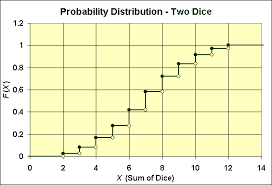
\includegraphics[width=0.7\linewidth]{cmf_dice.png}
	\caption{Cumulative distribution function for the sum obtained by rolling two dice}
	\label{fig:cmf_dice}
\end{figure}

\end{solution}
\begin{example}
Let $f(x) = c\left(\dfrac{1}{4}\right)^x$ be the pmf of the random variable $X$, where the support set is $\ZZ_{\geq 0}$ 
\begin{enumerate}
\item Find the appropriate constant $c$
\item Determine the cmf $F(x)$
\item Use the cmf to compute $\Pr[2 < X \leq 8]$
\item Write formulas involving $F$ and $f$ for the following
    \begin{enumerate}
        \item $\Pr[X > a]$
        \item $\Pr[X \geq a]$
        \item $\Pr[a < X < b]$
        \item $\Pr[a \leq X \leq b]$
    \end{enumerate}
\end{enumerate}
\begin{solution}
Most of the following analysis follows from definition: 
\begin{enumerate}
    \item Using the sum of an infinite geometric series formula, we arrive at $c = \frac 34$. 
    \item Using the sum of a finite geometric series formula, we arrive at $F(x) = \frac{3}{4}\left(\frac{1-(1/4)^{x+1}}{1-1/4}\right) = 1-(1/4)^{x+1}$
    \item $\Pr[2 < X \leq 8] = F(8)-F(2) = \frac{4095}{262144}$, from the cmf in b
    \item This is a more general question that applies to other cmfs other than this one: 
    \begin{enumerate}
        \item $\Pr[X > a] = 1-F(a)$
        \item $\Pr[X \geq a] = 1-F(a)+f(a) = 1-F(a)+\displaystyle\lim_{\Delta t \to 0} (F(a)-F(a-\Delta t))$
        \item $\Pr[a < X < b] = F(b)-F(a)-f(b) = F(b)-F(a)-\displaystyle\lim_{\Delta t \to 0} (F(b)-F(b-\Delta t))$
        \item $\Pr[a \leq X \leq b] = F(b)-F(a)+f(a)=F(b)-F(a)+\displaystyle\lim_{\Delta t \to 0} (F(a)-F(a-\Delta t))$
    \end{enumerate}

    % remark: the cmf is like the ``integral'' of f, if a ``derivative'' of F gives f?
\end{enumerate}
\end{solution}
\begin{remark}
Please note that what we are calling the cmf is very often called a \textbf{distribution function} in other texts and even by us, later on. The reasons will become more apparent when we extend pmf and cmf to continuous functions and partly-continuous functions.
\end{remark}
\end{example}

\section{Discrete Joint Probability Functions}

When two or more random experiments occur simultaneously, the 
outcomes can be analyzed with the use of a \textit{joint probability
function}. A common example is the height, $X$,  and weight, $Y$, of randomly selected subjects. If the subjects are humans, the sample space of $X$ (in feet) could 
be $\Omega_X = [0,10]$ and weight $\Omega_Y = [0,1000]$ in pounds.\footnote{These
sample spaces are discrete technically because of the finite limitation
of measurement, but for all practical purposes would best be treated as
continuous. The type doesn't concern us here; it's still a nice example.}

If enough sample data were collected, one could approximate $\Pr[X \dsp x \cap Y \dsp y]$ for $(x,y)$ in the joint sample space $\Omega_X \times
\Omega_Y$. This probability defines the joint probability function, or joint pmf:
$$f(x,y) = \Pr[X \dsp x, Y \dsp Y]$$
where the "comma" in the probability implies intersection and is usually read as "and." Be careful to \textbf{not} equate this with $\Pr[X \dsp x]\cdot\Pr[Y \dsp y]$, which would equal $\Pr[X \dsp x, Y \dsp Y]$
only when $X$ and $Y$ are independent. In fact, we should all be able to agree that height and weight of humans (or any type of object) are
almost always correlated and, therefore, \textit{not} independent.

The joint pmf of a set of discrete random variables $\{X_1, \ldots, X_n\}$
satisfies the following properties:
\begin{theorem} If $f$ is a function then $f$ can be the pmf of a set of random variables if and only if
\begin{eqnarray}
     f(x_1,\ldots,x_n) &\geq& 0 \\
    \sum_{x_1}\cdots\sum_{x_n}f(x_1,\ldots,x_n) &=& 1
\end{eqnarray}
Where in both items the sum is taken over all values in the domain of $f$.
\end{theorem}

\begin{example}
Let $f(x,y) = kxy$ be a pmf for $x=1,2,3$ and $y=1,2,3$. Determine the value of $k$
\end{example}

\begin{example}
A jar contains 3 red, 2 green and 4 blue marbles. Two marbles are drawn simultaneously at random. Let $R$ be the number of red and $G$ the number
of green marbles drawn. Determine the joint pmf $f(r,g)$
\label{ex:jar}
\end{example}

\begin{example}
Given the pmf $f(x,y,z)$ of random variables $X,Y,Z$
$$f(x,y,z) = \frac{(x+y)z}{63}\qquad x=1,2; y=1,2,3; z=1,2$$
calculate $\Pr[X \dsp 2, Y+Z \leq 3]$.
\end{example}

The last example hints at a definition for the cumulative
distribution function for a pmf $f$. In the bivariate case the definition is
\begin{definition}
Let $f(x,y)$ be the pmf of two random variables $X$ and $Y$. Then the distribution function $F(x,y)$ is defined by
$$F(x,y) = \Pr[X \leq x, Y \leq y] = \sum_{u=-\infty}^x \sum_{v=-\infty}^y f(u,v)$$
\end{definition}
\begin{example}
Determine the distribution function $F$ for the pmf defined in Example~\ref{ex:jar}
\end{example}
\begin{example}
Write an expression for $\Pr[a<X\leq b, c< Y \leq d$] in terms of $F$. Be 
careful to consider all the cases!
\end{example}

\subsection{Marginal and Conditional Distributions}
\end{document}
